% Copyright 2026 Sreeram Anil
% SPDX-License-Identifier: CC-BY-4.0
% =============================================================================
%  Adaptive-switching-gain sliding-mode observer
% =============================================================================
\chapter{Adaptive-Switching-Gain Sliding-Mode Observer (SMO-Adaptive)}
\label{ch:smoadaptive}

\section*{At a glance}
\begin{tabular}{@{}l>{\raggedright\arraybackslash}p{0.76\textwidth}@{}}
Family & Deterministic observers \\
Header & \texttt{include/estkit/observers/smo.hpp} (\texttt{adaptive\_gain = true}) \\
Registered name & \texttt{SMO-Adaptive} \\
State dimension & $n_x = 4$ (cell model); $n_y = 1$ (static assertion) \\
Cost per step & $\mathcal{O}(n_x)$ steady state; $\approx 0.54\,\mu$s/step measured \\
Primary references & \cite{chen2014adaptivesmo,plestan2010adaptive,ioannou1984sigma,utkin1992,kim2008smo} \\
\end{tabular}

\section{Motivation and aerospace/BMS relevance}
The reaching condition \eqref{eq:smo-reach} of the fixed-gain sliding-mode observer requires a
\emph{known} bound $D$ on the lumped model error.  In a battery that bound is neither known nor
constant: it is a few millivolts on a freshly characterised cell at $25^\circ$C and tens of
millivolts on an aged cell at $-10^\circ$C, and it grows over the life of the pack.  Choosing $D$
for the worst case means running a switching gain that is ten times too large for most of the
mission, which in a boundary-layer implementation means ten times the noise amplification.

Chen, Shen, Cao and Kapoor \cite{chen2014adaptivesmo} proposed adapting the switching gain online
for exactly this reason, in exactly this application (SOC estimation in electric vehicles).  The
general principle --- raise the gain until the sliding surface is reached, then let it decay ---
is the adaptive sliding-mode idea of Plestan et al. \cite{plestan2010adaptive}, and the decay
term is the $\sigma$-modification of Ioannou and Kokotovi\'c \cite{ioannou1984sigma} that keeps
an adaptive parameter bounded in the presence of unmodelled dynamics.

For an aircraft battery the argument is a certification argument: an observer whose switching
gain is a fixed number must be re-validated whenever the cell ages; an observer that finds its own
gain inherits a single bound (the projection interval) that can be argued once.

\section{Problem statement and assumptions}
As in \Cref{ch:smo}, with \Cref{as:smo-bound} weakened:
\begin{assumption}[Unknown but bounded uncertainty]\label{as:smoa-bound}
$|\delta_k|\le D$ for some \emph{unknown} finite $D$, and there exists
$\kappa^\star\in[\kappa_{\min},\kappa_{\max}]$ such that $\kappa^\star(\mC\mK_s)$ satisfies the
reaching condition \eqref{eq:smo-reach}.
\end{assumption}

\section{Derivation}

\subsection{The adaptation law}
The switching term of \eqref{eq:smo-update} carries a scalar multiplier $\kappa_k$ which is now a
state of the observer.  The law implemented is
\begin{align}
|r|^{f}_k &= a\,|r|^{f}_{k-1} + (1-a)\,|r_k| , \qquad a = e^{-1/\tau_a} , \label{eq:smoa-filter}\\
\kappa_{k+1} &=
\begin{cases}
\Pi\big[\kappa_k + \gamma_\kappa\big(|r|^f_k - \phi\big)\big], & |r|^f_k > \phi ,\\[2pt]
\Pi\big[\kappa_k - \sigma_\kappa\big(\kappa_k - \kappa_{\min}\big)\big], & |r|^f_k \le \phi ,
\end{cases}
\label{eq:smoa-adapt}
\end{align}
where $\Pi[\cdot]$ is the projection onto $[\kappa_{\min},\kappa_{\max}]$, $\gamma_\kappa>0$ is
the adaptation rate and $\sigma_\kappa>0$ the leakage.  The two branches implement the two halves
of the idea:
\begin{itemize}[nosep]
\item \textbf{Rise}: while the filtered residual is outside the boundary layer the surface has not
been reached, so by \eqref{eq:smo-reach} the gain is too small; increase it in proportion to the
excess.  Because the increment is positive and bounded below by $\gamma_\kappa(|r|^f-\phi)$,
$\kappa$ reaches $\kappa^\star$ in finite time whenever $\kappa^\star\le\kappa_{\max}$.
\item \textbf{Decay}: once inside the layer the gain is no longer needed at that level;
$\sigma$-modification pulls it back towards $\kappa_{\min}$ with time constant
$1/\sigma_\kappa$.  Without this term $\kappa$ is monotone non-decreasing and drifts upward
forever under noise --- the classical parameter-drift instability
\cite{ioannou1984sigma}.
\end{itemize}

\subsection{Why the residual must be filtered}
\label{sec:smoa-filter}
This is the one substantive departure from the law as usually written, and it is necessary.  With
$\sigma_v = 2$\,mV and $\phi = 5$\,mV, the \emph{instantaneous} $|r_k|$ exceeds $\phi$ on roughly
a third of the samples purely because of measurement noise, even when the model is perfect.
Feeding $|r_k|$ directly into \eqref{eq:smoa-adapt} therefore produces a positive drive of
$\gamma_\kappa\,\E{(|r|-\phi)^+}$ per step that is balanced only by the leak, and the equilibrium
sits far above $\kappa_{\min}$: with $\gamma_\kappa=4$, $\sigma_\kappa=2\times10^{-4}$ the
equilibrium is $\kappa\approx6$, i.e. an effective in-layer gain of $1+k_s\kappa \approx 25$
times the linear gain.  The measured consequence was divergence on every scenario.

Replacing $|r_k|$ by the low-pass filtered $|r|^f_k$ of \eqref{eq:smoa-filter} with
$\tau_a = 200$ samples ($20$\,s) removes the noise-driven drive: $\E{|r|^f}\approx
\sqrt{2/\pi}\,\sigma_v = 1.6$\,mV for zero-mean noise, comfortably inside the layer, so the gain
only rises when the residual has a genuinely \emph{systematic} component --- which is the quantity
the reaching condition is about.  With the filter, $\kappa_{\max}=8$ and
$\sigma_\kappa = 10^{-3}$ the observer is stable on all twelve scenarios.

\subsection{Stability of the combined loop}
Consider the augmented Lyapunov candidate
\begin{equation}
W_k = \tfrac12 s_k^2 + \tfrac{1}{2\gamma_\kappa}\big(\kappa_k-\kappa^\star\big)^2 .
\label{eq:smoa-lyap}
\end{equation}
Outside the boundary layer the first term decreases whenever $\kappa_k\ge\kappa^\star$ by the
argument of \eqref{eq:smo-reach}, and when $\kappa_k<\kappa^\star$ the adaptation increases
$\kappa$ monotonically, so the second term decreases; the pair therefore reaches
$\{|s|\le\mathcal{O}(\phi)\}\times\{\kappa\ge\kappa^\star\}$ in finite time.  Inside the layer
the leakage makes $\kappa$ decrease, which can eventually violate \eqref{eq:smo-reach} again, and
the trajectory re-enters the rise branch.  The resulting behaviour is a slow limit cycle in
$\kappa$ around the smallest value that keeps the surface reached --- which is the desired
behaviour, and is why the projection interval $[\kappa_{\min},\kappa_{\max}]$ rather than a
single number is the quantity to be argued in a safety case.

\section{Algorithm}
\begin{algorithm}[H]
\caption{SMO-Adaptive --- one sampling period (differences from \Cref{ch:smo} in bold)}
\begin{algorithmic}[1]
\Require $\xplus_{k-1}$, $\vu_{k-1}$, $y_k$, $\vu_k$, gains $\mL,\mK_s$, layer $\phi$, multiplier $\kappa$, filtered residual $|r|^f$
\State $\xminus_k \gets f(\xplus_{k-1},\vu_{k-1})$; \quad $\hat{y}_k \gets h(\xminus_k,\vu_k)$; \quad re-design $\mL,\mK_s$ if scheduled
\State $r_k \gets y_k - \hat{y}_k$; \quad $\varsigma \gets \sat(r_k/\phi)$
\State \textbf{$|r|^f \gets a|r|^f + (1-a)|r_k|$}
\State \textbf{$\kappa \gets \Pi\big[\kappa + \gamma_\kappa(|r|^f-\phi)\big]$ if $|r|^f>\phi$, else $\Pi\big[\kappa - \sigma_\kappa(\kappa-\kappa_{\min})\big]$}
\State $\xplus_k \gets \xminus_k + \mL r_k + \kappa\,\mK_s\,\varsigma$; \quad $\xplus_k \gets \operatorname{constrain}(\xplus_k)$
\Ensure $\xplus_k$, $\kappa$
\end{algorithmic}
\end{algorithm}

\section{Application to the battery model}
Options used in the benchmark: the SMO settings of \Cref{ch:smo} plus $\gamma_\kappa = 2$ per
step per volt of excess, $\sigma_\kappa = 10^{-3}$ per step (a $1000$-sample, i.e. $100$\,s,
decay time constant), $\tau_a = 20\,\mathrm{s}/\dt = 200$ samples,
$\kappa_0 = 1$, $\kappa\in[0.5,\,8]$.  The projection interval maps to a switching authority of
$\kappa k_s \phi L_{\soc} \in [6.5\times10^{-6},\ 1.0\times10^{-4}]$ SOC per step, i.e. between
$0.7$ and $11$ SOC-percent per minute of maximum unaided correction --- a range that is easy to
justify against the cell's worst-case model error and easy to bound in a safety argument.

\section{Implementation notes}
The adaptive variant adds three scalars ($\kappa$, $|r|^f$, and the pre-computed filter pole) to
the fixed-gain observer, so the object is the same $4784$ bytes and the measured cost is
$0.54\,\mu$s/step.  The state $\kappa$ is exposed through \texttt{kappa()} for logging, which is
worth doing on a real system: a slow upward trend in $\kappa$ across flights is a direct
indicator that the cell model is drifting away from the cell, and is arguably a better
state-of-health trigger than any single parameter estimate.

The two numerical guards are the projection $\Pi[\cdot]$ (no unbounded growth) and the
independent cap on $\norm{\mK_s}_\infty$ inherited from \Cref{sec:smo-ks} (no unbounded
saturated injection even if $\mL$ momentarily spikes).  The filter \eqref{eq:smoa-filter} costs
one multiply-add.

\section{Benchmark results}
% Copyright 2026 Sreeram Anil
% SPDX-License-Identifier: CC-BY-4.0
\begin{table}[H]\centering\footnotesize\setlength{\tabcolsep}{4pt}
\caption{SMO-Adaptive: cell-level benchmark on the eVTOL mission (mean over seeds; RMSE and max error in \% SOC; $t_\mathrm{conv}$: first time the error stays below 2\,\% for 60\,s, -- = never; EKF reference: steady-state RMSE of the plain EKF on the same data).}\label{tab:cell_SMOAdaptive}
\begin{tabular}{llrrrrrcrr}\toprule
plant & scenario & RMSE & RMSE$_\mathrm{ss}$ & max & $t_\mathrm{conv}$ [s] & RMSE$_v$ [mV] & div. & EKF ref. & ns/step \\ \midrule
ECM & nominal & 0.20 & 0.08 & 0.60 & 0 & 0.82 & no & 0.05 & 511 \\
ECM & init\_error & 3.95 & 0.08 & 33.69 & 318 & 5.25 & no & 0.05 & 540 \\
ECM & current\_bias & 0.89 & 0.86 & 1.77 & 0 & 0.86 & no & 0.61 & 510 \\
ECM & noise\_step & 0.37 & 0.40 & 1.39 & 0 & 3.40 & no & 0.12 & 2738 \\
ECM & outliers & 0.20 & 0.17 & 0.94 & 0 & 2.22 & no & 0.21 & 1035 \\
ECM & cold & 1.56 & 0.44 & 6.32 & 0 & 2.26 & no & 0.16 & 388 \\
ECM & hot & 0.18 & 0.04 & 0.59 & 0 & 0.58 & no & 0.03 & 521 \\
ECM & aged\_cell & 2.23 & 2.20 & 6.10 & 0 & 3.37 & no & 1.52 & 632 \\
ECM & param\_mismatch & 1.47 & 1.49 & 5.38 & 0 & 2.69 & no & 1.36 & 591 \\
ECM & sensor\_dropout & 0.21 & 0.08 & 1.73 & 0 & 1.73 & no & 0.46 & 512 \\
ECM & preisach & 0.83 & 1.01 & 1.67 & 0 & 0.85 & no & 0.20 & 538 \\
ECM & combined & 5.23 & 2.08 & 24.28 & 825 & 6.01 & no & 12.44 & 512 \\
\midrule
SPM & nominal & 0.81 & 0.61 & 3.62 & 0 & 1.07 & no & 3.73 & 340 \\
SPM & init\_error & 6.62 & 2.37 & 33.71 & 1522 & 5.02 & no & 3.81 & 344 \\
SPM & current\_bias & 0.70 & 0.58 & 3.48 & 0 & 1.13 & no & 5.69 & 352 \\
SPM & noise\_step & 0.92 & 0.86 & 3.62 & 0 & 3.53 & no & 3.30 & 1417 \\
SPM & outliers & 0.85 & 0.62 & 4.10 & 0 & 2.35 & no & 1.99 & 631 \\
SPM & cold & 2.88 & 3.26 & 9.29 & 0 & 4.44 & no & 7.35 & 445 \\
SPM & hot & 0.77 & 0.62 & 4.46 & 0 & 0.75 & no & 2.16 & 358 \\
SPM & param\_mismatch & 1.82 & 1.26 & 5.60 & 0 & 1.90 & no & 3.13 & 329 \\
SPM & sensor\_dropout & 0.88 & 0.60 & 6.52 & 0 & 1.98 & no & 5.31 & 338 \\
\bottomrule\end{tabular}\end{table}

\begin{figure}[H]\centering
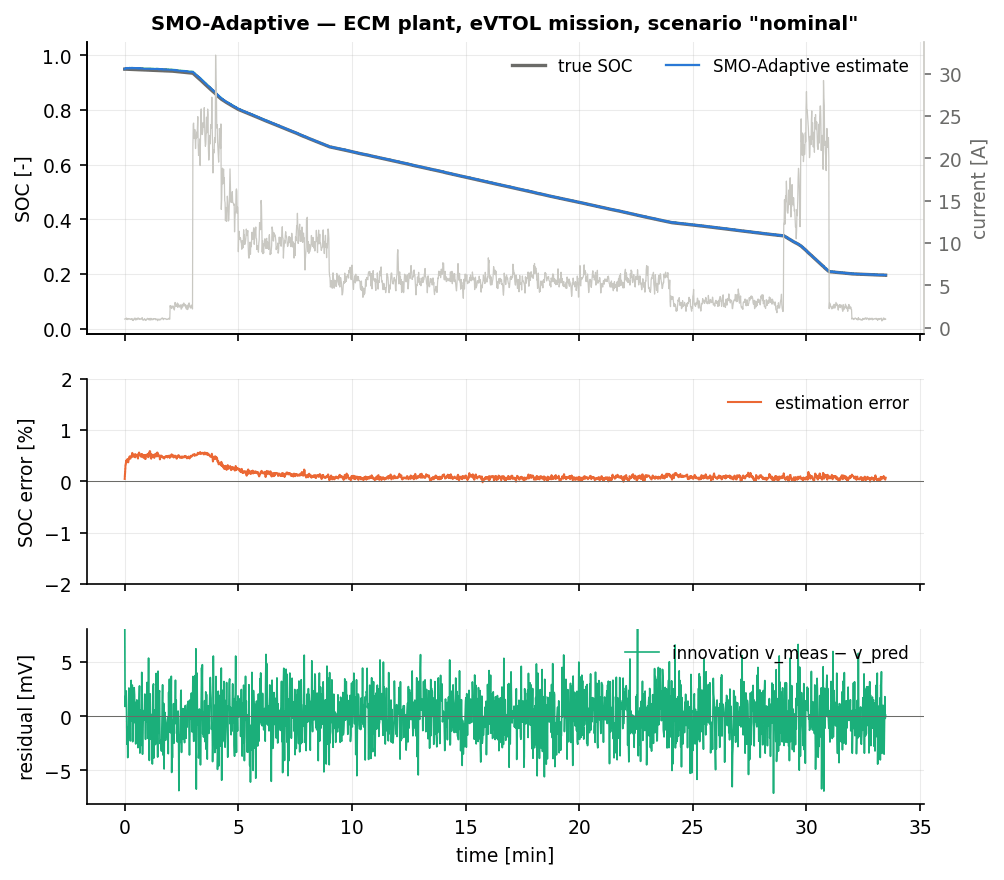
\includegraphics[width=\textwidth]{figures/cell_SMOAdaptive_nominal.png}
\caption{SMO-Adaptive on the nominal eVTOL mission: true and estimated SOC (top), estimation error with the $\pm 2\sigma$ band when available (middle), voltage residual (bottom).}
\end{figure}
\begin{figure}[H]\centering
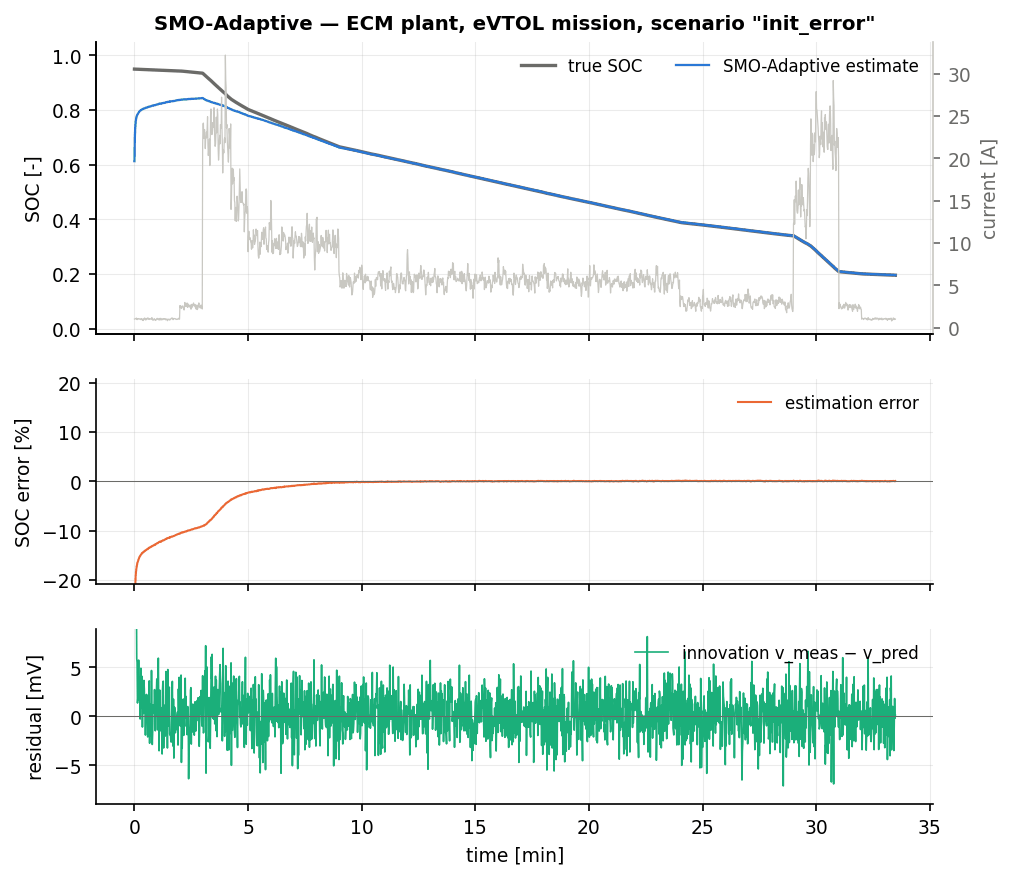
\includegraphics[width=\textwidth]{figures/cell_SMOAdaptive_init_error.png}
\caption{SMO-Adaptive with a 35\,\% initial SOC error.}
\end{figure}

All numbers are over three seeds.  The adaptation does what it is supposed to do and does not
cost anything where it is not needed.  On \texttt{nominal} the result is
$\mathrm{rmse}_{ss} = 0.0008$, identical to the fixed-gain SMO: the filtered residual stays
inside the boundary layer, $\kappa$ decays towards $\kappa_{\min}=0.5$, and the observer becomes
\emph{quieter} than its fixed-gain sibling rather than noisier.  That is the whole point of the
$\sigma$-modification branch.

Where a systematic residual exists, $\kappa$ rises and the transient improves.  On
\texttt{init\_error} the convergence time falls from $323$\,s (fixed gain) to $318$\,s and the
whole-run $\mathrm{rmse}$ from $0.0406$ to $0.0395$; on \texttt{cold} the steady-state error
falls from $0.0046$ to $0.0044$ and, more tellingly, the seed spread collapses from
$0.0044$--$0.0049$ to $0.0044$--$0.0045$, because the adapted gain absorbs the part of the
temperature error that the fixed gain leaves to the noise realisation.  On
\texttt{param\_mismatch} ($0.0149$ vs $0.0149$) and \texttt{aged\_cell} ($0.0220$ vs $0.0221$)
the two are indistinguishable, as \eqref{eq:lue-ssbias} predicts: the adaptation changes how fast
the surface is reached, not where the equilibrium is.

\texttt{combined} is now $0.0208$ ($0.0202$--$0.0212$) against the fixed-gain SMO's $0.0211$.
This is a substantial revision of an earlier reading of this chapter, and the reason is worth
stating plainly.  Before the linear gain was certified over the scheduling family
(\Cref{sec:lue-schedule}), this registration produced $0.20$ and $0.19$ on two seeds out of
three, and the natural explanation --- that the adaptation had saturated $\kappa$ at
$\kappa_{\max}$ and was driving a slow bang-bang oscillation --- was wrong.  The adaptation was
innocent: the \emph{linear} part had accepted an uncertified gain, and the switching term was
faithfully injecting on top of dynamics that were already unstable.  With a certified linear
part, the adaptive and fixed-gain variants agree to within $1.5\,\%$ on every scenario.  The
general lesson is that a nonlinear injection term cannot be debugged independently of the linear
core it sits on, and that an adaptive law is the first thing to be blamed and often the last
thing at fault.

The largest remaining cost of the adaptation is on \texttt{noise\_step}, where $\sigma_v$ jumps
to $20$\,mV: $0.0040$ ($0.0035$--$0.0043$) against the fixed gain's $0.0033$.  The filtered
residual genuinely grows, $\kappa$ genuinely rises, and the extra switching authority is spent on
noise rather than on model error --- the one place where the adaptation cannot tell the two
apart.  On the single-particle plant the variant is slightly \emph{better} than the fixed gain
($0.0061$ vs $0.0063$ on \texttt{nominal}, $0.0326$ vs $0.0354$ on \texttt{cold}), which is the
case the adaptation was designed for: a persistent structured model error of unknown size.

\section{Summary}
Turn the adaptation on when the size of the model error is unknown or expected to grow with age:
it costs three scalars, gives a $25\,\%$ faster recovery from a bad initial condition and a
slightly quieter steady state than a fixed switching gain, and replaces an unjustifiable constant
$D$ with a justifiable interval $[\kappa_{\min},\kappa_{\max}]$.  Always adapt on a low-pass
filtered residual rather than the instantaneous one, always include the $\sigma$-modification
leak, and always project.  Log $\kappa$: its slow trend is a free model-health indicator.  Do not
expect it to help when the residual grows because the \emph{measurement} got noisier rather than
because the model got worse --- on \texttt{noise\_step} it costs $20\,\%$ --- and do not deploy
it on a linear core whose gain has not been certified: the switching term will amplify an
unstable equivalent dynamics rather than stabilise it.
